\subsection{Use Cases}
For at sikre at vi laver et program, der fungerer som ønsket, har vi opstillet flere use cases for systemet.
Disse use cases er blevet udledt på baggrund af møder med Psykolog Nords ledelse, og ved brug af de fire basis funktioner for persistens: create, read, update og delete (CRUD), på objekt- og domænemodelen.
Derudover har vi også identificeret primæraktørene og deres mål, og sikret at vores use cases opfylder målene.

Vores primæraktører og deres mål er:

\begin{itemize}
    \item Booking ansvarlig
        \begin{itemize}
            \item Se aftaler
            \item Book aftale
            \item Ændr aftale
            \item Aflys aftale
        \end{itemize}
    \item Psykolog
        \begin{itemize}
            \item Ajourfør kundes journal
        \end{itemize}
    \item Kunde
        \begin{itemize}
            \item Se og betal fakturaer
            \item Book aftale
            \item Ændr aftale
            \item Aflys aftale
        \end{itemize}
    \item Superbruger
        \begin{itemize}
            \item Håndter bruger
            \item Håndter brugers rettigheder
        \end{itemize}

\end{itemize}

Det er f.eks. vigtigt at skelne mellem at booke en ny aftale, ændre den og aflyse den, da det er tre forskellige funktionaliteter i systemet.

\begin{figure}[p]
	\centering
  		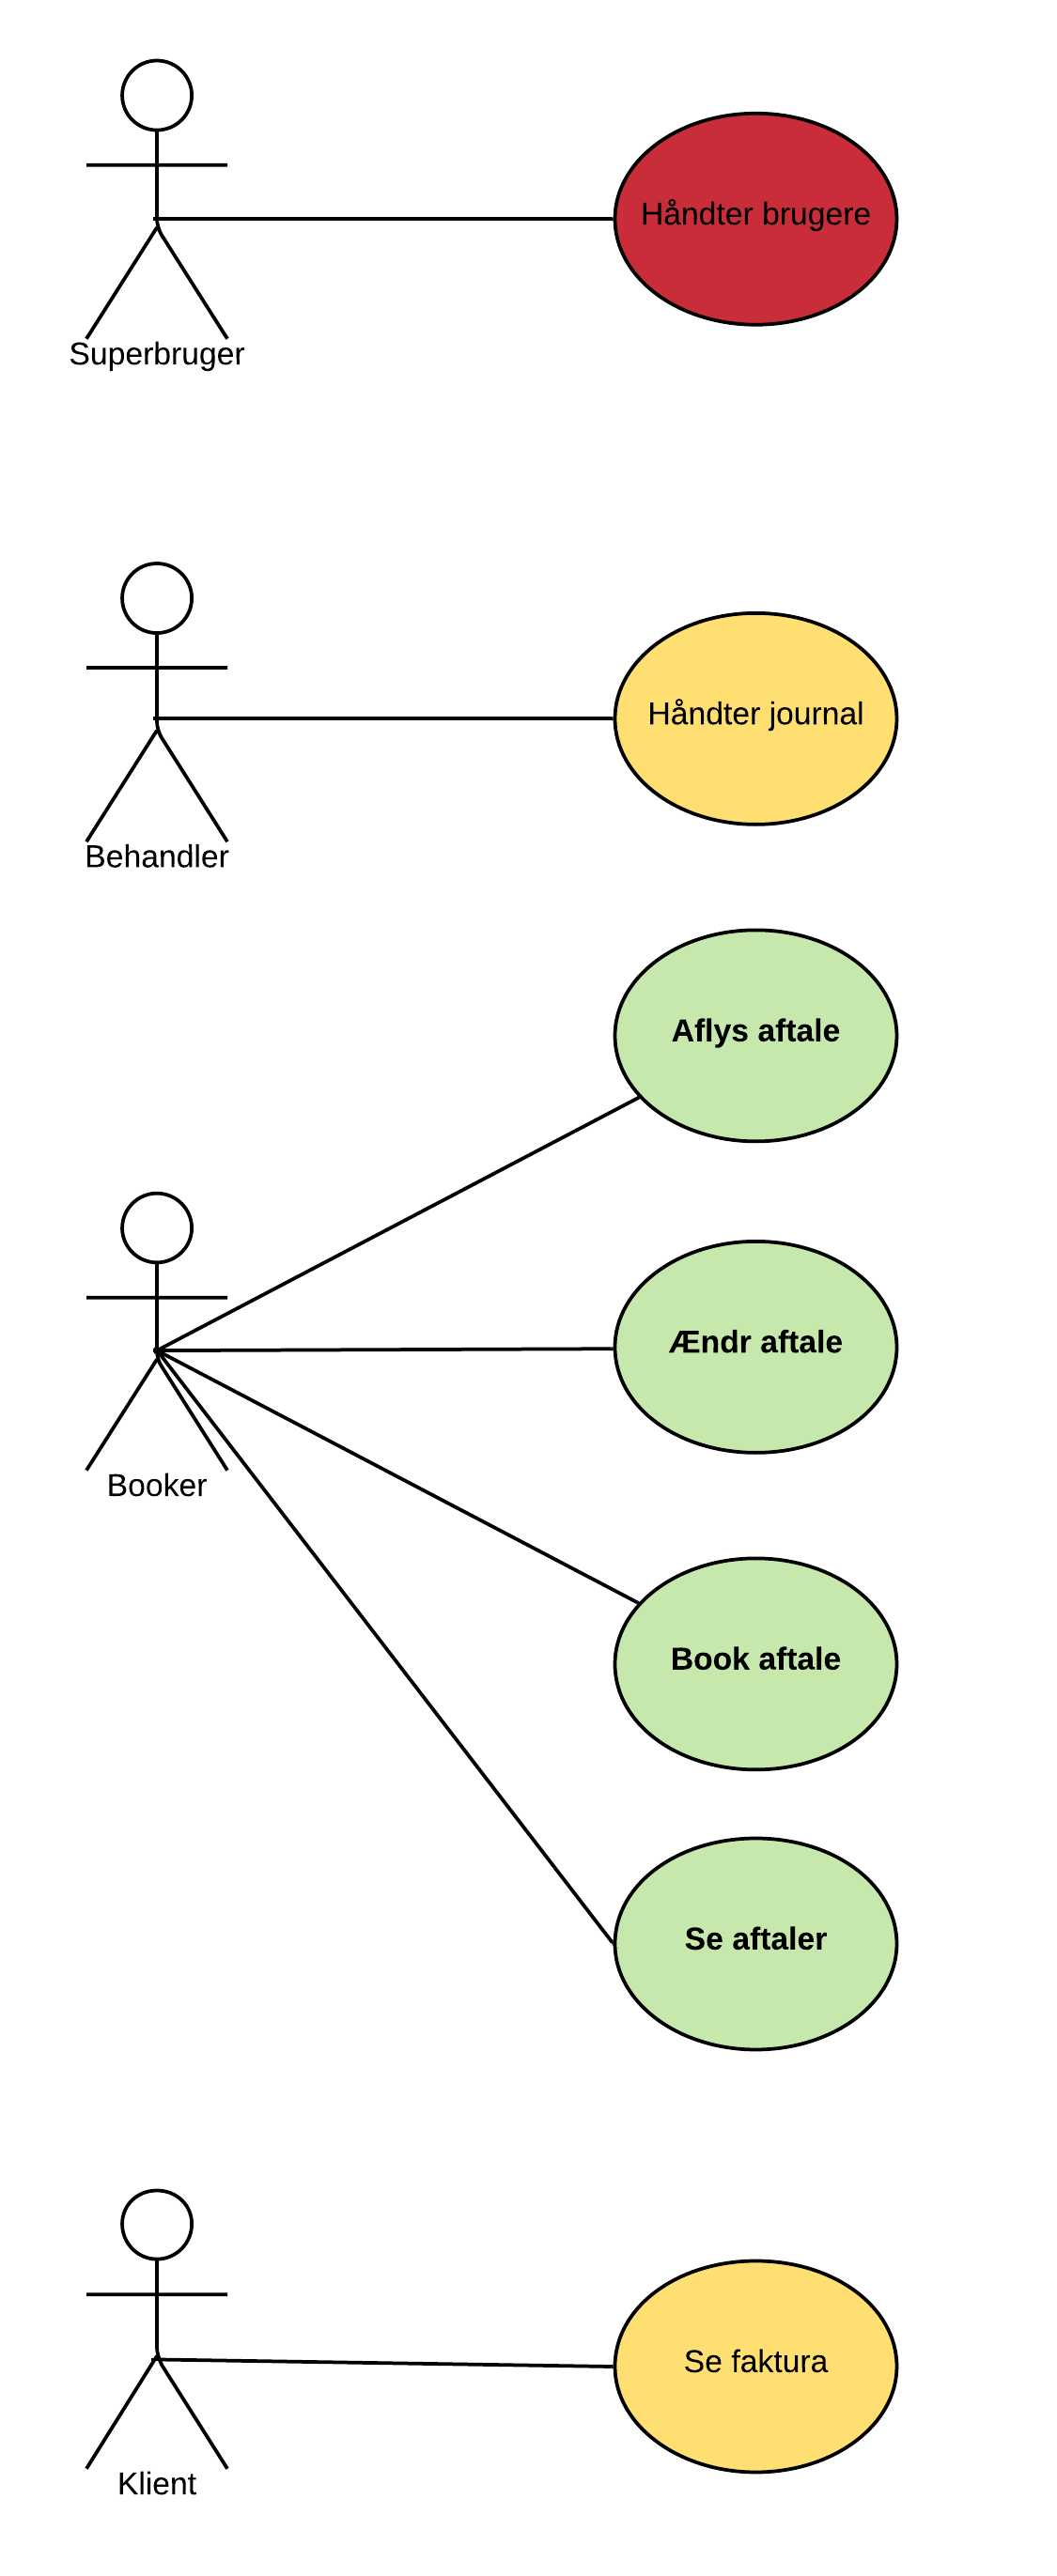
\includegraphics[scale=0.75]{UseCaseDiagram.png}
  \caption{Use Case diagram.}
  \label{fig:UseCaseDiagram}
\end{figure}

På figur \ref{fig:UseCaseDiagram} kan man se alle de use cases vi fandt frem til.
Uses casesne er blevet markeret med farver, der repræsenterer deres prioritering under projektforløbet: de grønne var dem, som Psykolog Nord først ønskede implementeret, derefter gul og tilsidst grøn.
I følgende kapitel kan man så findes vores use cases beskrevet mere detaljeret. 

To personer deltager i en aftale: en kunde og en psykolog.

\subsubsection{Use Case: Book aftale}\label{usecase:bookaftale}
{\setlength{\parindent}{0cm}
\textbf{Scope:} Bookingsystem for Psykolog Nord

\textbf{Primær Aktør:} Bookingansvarlig

\textbf{Hovedscenarie (succes):} Booking af ny aftale

Den bookingansvarlige ønsker at booke en aftale.
Hvis den involverede kunde ikke har brugt PsykologNord før, oprettes kunden i systemet.
Kunden vælger aftaletype og der bookes en ny aftale, hvor både kunden og psykologen har tid. 
Aftalen bookes og kunde og psykolog notificeres.

\textbf{Primær Aktør:} Kunde og bookingansvarlig

\textbf{Alternativt scenarie (succes):} Kontakt PsykologNord for at booke en aftale

En kunde ønsker at booke en aftale, og kontakter derfor PsykologNord.
En bookingansvarlig booker aftalen som i hovedscenariet.

\textbf{Primær Aktør:} Kunde

\textbf{Alternativt scenarie (succes):} Vælge Parterapi som aftale

En kunde ønsker at booke en parterapi aftale.
Hvis den involverede kunde ikke har brugt PsykologNord før, oprettes kunden i systemet.
Kunden vælger aftaletype, og indtaster den anden kundes informationer, og den anden kunde oprettes også i systemet.
Der bookes en ny aftale, hvor både kunden og psykologen har tid. 
Aftalen bookes, begge kunder og psykologen notificeres.
}

\subsubsection{Use Case: Ændr Aftale}
{\setlength{\parindent}{0cm}
\textbf{Scope:} Bookingsystem for Psykolog Nord

\textbf{Primær Aktør:} Booking ansvarlig 

\textbf{Preconditions:} En aftale eksisterer, og der er mere end 24 timer til aftalen.

\textbf{Hovedscenarie (succes):} Ændring af aftale

Den bookingansvarlige går ind i systemet og ændrer aftalen til andet tidspunkt, hvor kunden og psykologen kan.
Kunde og psykolog modtager en notifikation med ændringen.

\textbf{Primær Aktør:} Kunde og bookingansvarlig

\textbf{Alternativt scenarie:} Kunde ændrer aftale ved at kontakte PsykologNord.

Kunden ønsker at ændre sin aftale, og kontakter derfor PsykologNord.
En bookingansvarlig ændrer aftalen som i hovedscenariet.
}

\subsubsection{Use case: Aflys Aftale}
{\setlength{\parindent}{0cm}
\textbf{Scope:} Bookingsystem for Psykolog Nord

\textbf{Primær Aktør:} Bookingansvarlig

\textbf{Preconditions:} En aftale eksisterer.

\textbf{Hovedscenarie (succes):} Aflysning af aftale

Den bookingansvarlige aflyser aftalen.
Den involverede kunde og psykolog modtager en besked om aflysningen. Fakturaen, der er tilkoblet aftalen, slettes.

\textbf{Primær Aktør:} Kunde og bookingansvarlig

\textbf{Alternativt scenarie:} Kunde aflyser aftale ved at kontakte PsykologNord.

En kunde ønsker at aflyse en aftale og kontakter derfor PsykologNord.
Den bookingansvarlige aflyser aftalen som i hovedscenariet.

\textbf{Primær Aktør:} Kunde

\textbf{Alternativt scenarie:} Aflysning af aftale med mindre end 24 timer til aftales start

Kunden ønsker at aflyse en aftale, der er mindre en 24 timer til.
Psykologen modtager en notifikation om aflysningen, men fakturaen sendes stadig til klienten.
}

\subsubsection{Use Case: Se og betal faktura}
{\setlength{\parindent}{0cm}
\textbf{Scope:} Bookingsystem for Psykolog Nord

\textbf{Primær Aktør:} Klient

\textbf{Precondition:} Faktura eksisterer.

\textbf{Hovedscenarie (success):} Se faktura

Klienten går ind i systemet og finder listen over fakturaer. 
Han finder den ønskede faktura og får den vist. Klienten betale derefter fakturaen og modtager kvittering.
}

\subsubsection{Use Case: Ajourfør kundes journal}
{\setlength{\parindent}{0cm}
\textbf{Scope:} Bookingsystem for Psykolog Nord

\textbf{Primær Aktør:} Psykolog

\textbf{Precondition:} Kunde eksisterer og har været til aftale.

\textbf{Hovedscenarie (success):} Ajourfør kundes journal

En psykolog ønsker at ajourføre en af sine kunders journaler.
Psykologen tilgår sin kundeoversigt og vælger den ønskede kunde.
Psykologen ser nu en oversigt over sin kundes journalindlæg, og psykologen laver et nyt journalindlæg og tilføjer sine notater.
}
